\section{A Smarter $\chi^2$}
\label{891_2:sec:smart_chi}

The algorithms used for full-spectrum fitting are designed to minimize
the $\chi^2$ difference between some model spectrum and our
observational data. In this $\chi^2$ calculation each wavelength
channel is given a weight equal to the inverse of the poisson noise
propagation described in section \ref{891_2:sec:data}. This type of
weighting benefits from historical momentum and ease of implementation
but ignores the fact that certain wavelength regions are
astrophysically more important than others for constraining star
formation histories. In other words, a traditional $\chi^2$
calculation gives more-or-less equal weight to all wavelength channels
despite the fact that some channels are more sensitive to differences
in models than others.

%% {\bf MAB: my question about the above paragraph is if it is true that
%%   everyone is basically using $\chi^2$ for FSF. Have you checked the
%%   literature?}

% ADE: Yes, and yes. Doesn't seem necessary to ref though

To capture this astrophysical importance we compute a weighting
spectrum that is applied to $\chi^2$ during full-spectrum
fitting. These weights are computed as the root-means-square (RMS)
difference between the model basis SSPs and therefore capture how much
each wavelength channel changes with different SSPs. For this
calculation we use the \val{0.2}{\Zsol}, \val{0.4}{\Zsol},
\val{1}{\Zsol}, and \val{2.5}{\Zsol} mono-metallicity
\citetalias{Bruzual03} diffusion k-means SSPs (see section
\ref{891_2:sec:bc03_dfk}).

%++++++++++++++++
%% {\bf MAB: by ``additional weights'' you should clarify that they are
%%   in addition to the error weights.}

Before computing the RMS, each SSP is normalized to have a flat
continuum to remove any low-order continuum shape effects from the
final weights. This step is important because the continuum shape
changes significantly with different metallicities and ages and also
because the overall continuum shape in the full-spectrum fits is
controlled largely by the extinction parameter, \tauV. The average
spectrum across all ages and metallicities is then computed and set as
the zero point for computing the final RMS spectrum. This attempt to
remove the effects of low-order spectral shape is similar to the
method of FIREFLY \citep{Wilkinson15}.

%+++++++++++
%% {\bf MAB: This would be a nice opportunity to mention FIREFLY. In
%%   essence we are looking to acheieve what they did but w/o filter the
%%   data. The only concern with saying this might be the referee asking
%%   why we didn't use FIREFLY.}

\begin{figure}
  \centering
  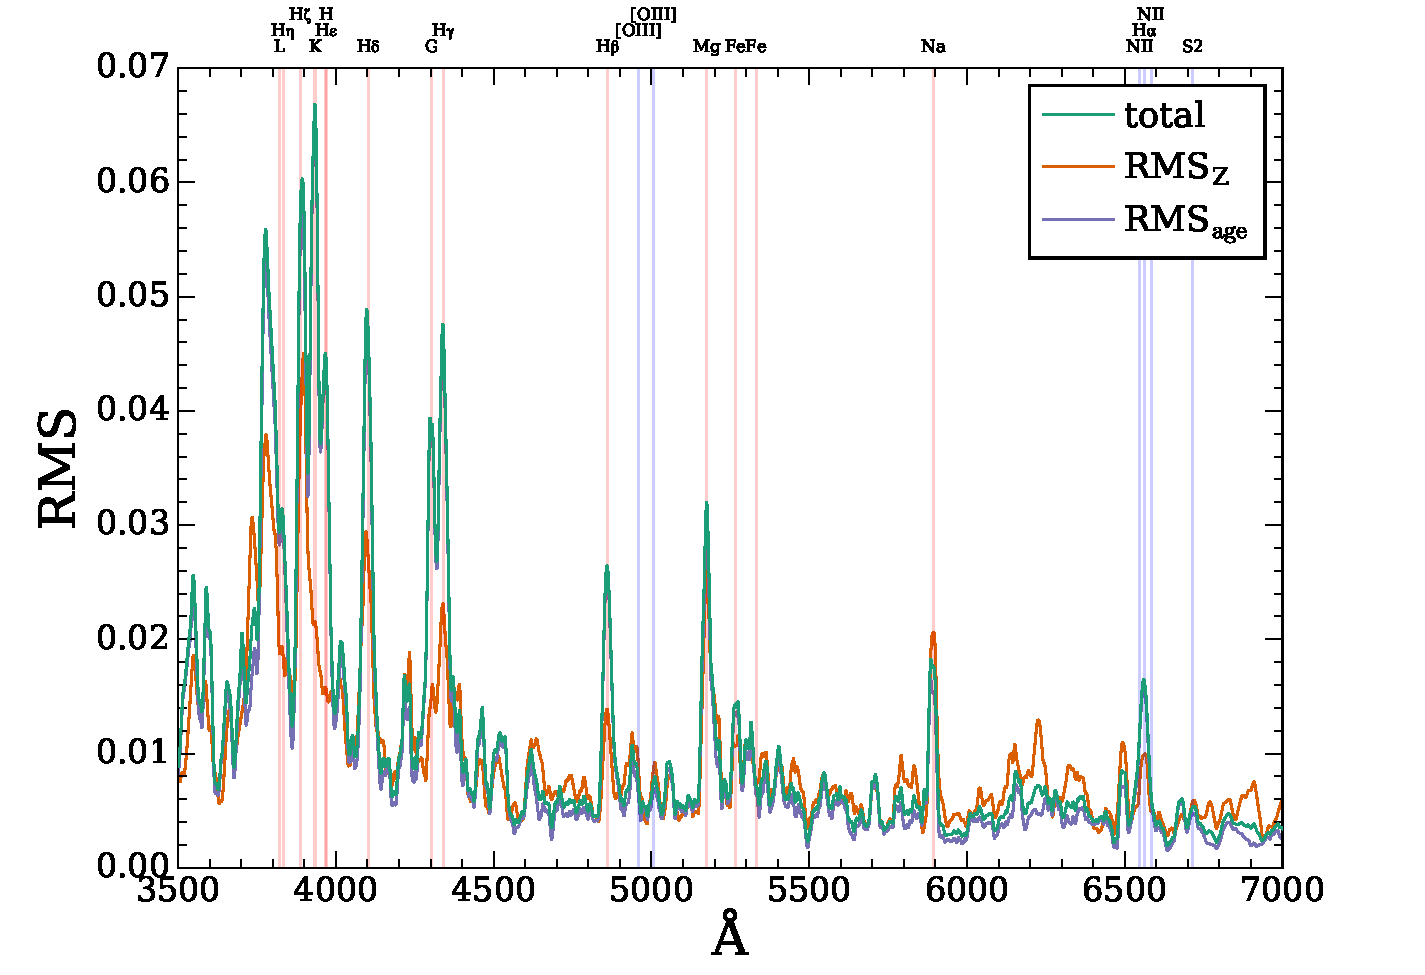
\includegraphics[width=\columnwidth]{891_2/figs/RMS_spec.pdf}
  \caption[RMS-based $\chi^2$ fitting
    weights]{\fixspacing\label{891_2:fig:RMS_spec}The RMS weighting
    function used to modify our $\chi^2$ fits ($R(\lambda)$ in
    Equation. \ref{891_2:eq:smart_chi}). The total RMS value is
    computed across all metallicities and ages. RMS$_Z$ is computed
    across all metallicities and is sensitive to differences between
    models with different metallicity values. Similarly,
    RMS$_\mathrm{age}$ is computed across all ages and is therefore
    more sensitive to model differences as a function of age.}
    %% The red line is the same as the
    %% green, but computed across all metallicities. The red and green
    %% lines show the quadrature sum of the individual RMS$_Z$ or
    %% RMS$_{age}$ computed across all ages or metallicities,
    %% respectively \textbf{this is almost certainly not clear}. Vertical
    %% lines show important emission (blue) and absorption (red)
    %% features.}
\end{figure}

Figure \ref{891_2:fig:RMS_spec} shows the resulting RMS spectrum along
with important spectral features. In addition to computing the RMS
across all ages and metallicities we also compute RMS spectra across
all ages at each metallicity and vice versa. The ``total'' RMS closely
matches the RMS across age, which suggests that age variations cause
the majority of the difference between different SSPs. There are also
few spectral features that are have a high RMS value in \emph{only}
age or metallicity, which suggests these weights will struggle to
break the age/metallicity degeneracy.

The total RMS spectrum modifies the traditional $\chi^2$ by
\begin{equation}
\label{891_2:eq:smart_chi}
\chi^2 = \sum_{\lambda}\left(\frac{f(\lambda) -
  g(\lambda)}{\sigma(\lambda)}\zeta(\lambda)\right)^2,
\end{equation}
where $f(\lambda)$ and $g(\lambda)$ are the data and model spectra,
respectively, $\sigma(\lambda)$ is the poisson errors on $f(\lambda)$, and
$\zeta(\lambda)$ is the RMS spectrum.

%+++++++++++++
%% {\bf MAB: Discuss how to read the figure since it is almost impossible
%%   to make out the $RMS_{age}$ line. I think you want to say that is is
%%   easiest to make out the ``total'' (green) and Z (orange) curves
%%   which demonsrates that in most cases where there are strong peaks
%%   age variations dominates, particularly below 4500 \AA\. Redward
%%   there are weaker features where Z dominates. However, at every
%%   location where there is a strong peak in RMS both age and Z increase
%%   (except perhaps for Ca HK, which is weird), which already
%%   foreshadows that this weighting scheme is not going to bust the
%%   age-Z degeneracy.}


In addition to modifying our full-spectrum fits, the results shown in
Figure \ref{891_2:fig:RMS_spec} provide insight into the statistically
important differences between model spectra. The Balmer series stands
out as strong indicators of both age and metallicity, but surprisingly
the higher-order Balmer lines (\Hd, \Hg) have more power than \HB and
\Ha. This is important because in the absence of an accurate
correction for Balmer emission (\S\ref{891_2:sec:emission_corr}) these
higher order lines are less likely to be contaminated. Beyond the
Balmer series Na, Fe, Mg, and G-band absorption also have powerful
spikes in the RMS spectrum. Unfortunately the distance to NGC 891
places Na absorption right on top of the NaD sky emission line so it
cannot be used in analysis. 

In many ways the index/equivalent width measurements common to
Astronomy and used in Chapter \ref{chap:891_1} can be thought of as
$\chi^2$ comparisons that are very highly tuned to specific spectral
features and therefore are highly dependent on the stellar physics
that go into producing the models. In this context it comes as no
surprise that the spectral features that differentiate our SSP models
are the same features that have been used extensively in the LICK
system to assign astrophysical parameters to observations of galaxy
and stars.

%+++++++++++++++++
%% {\bf MAB: This is a good discussion. I am trying to think whether it
%%   is surprising that \Hd and \Hg have more variation than \HB and \Ha.
%%   This may be well known, but the point about the emission correction
%%   is a good one. Note NaD also problematic because of ISM within the
%%   external galaxy. Concerning ``a ton of people'' just reference the
%%   Lick system and either give no reference or cite something like
%%   Burstein 1984.}

\begin{figure*}[t]
  \centering
%  \includegraphics[width=\textwidth]{891_2/figs/weight_comp_sys.pdf}
  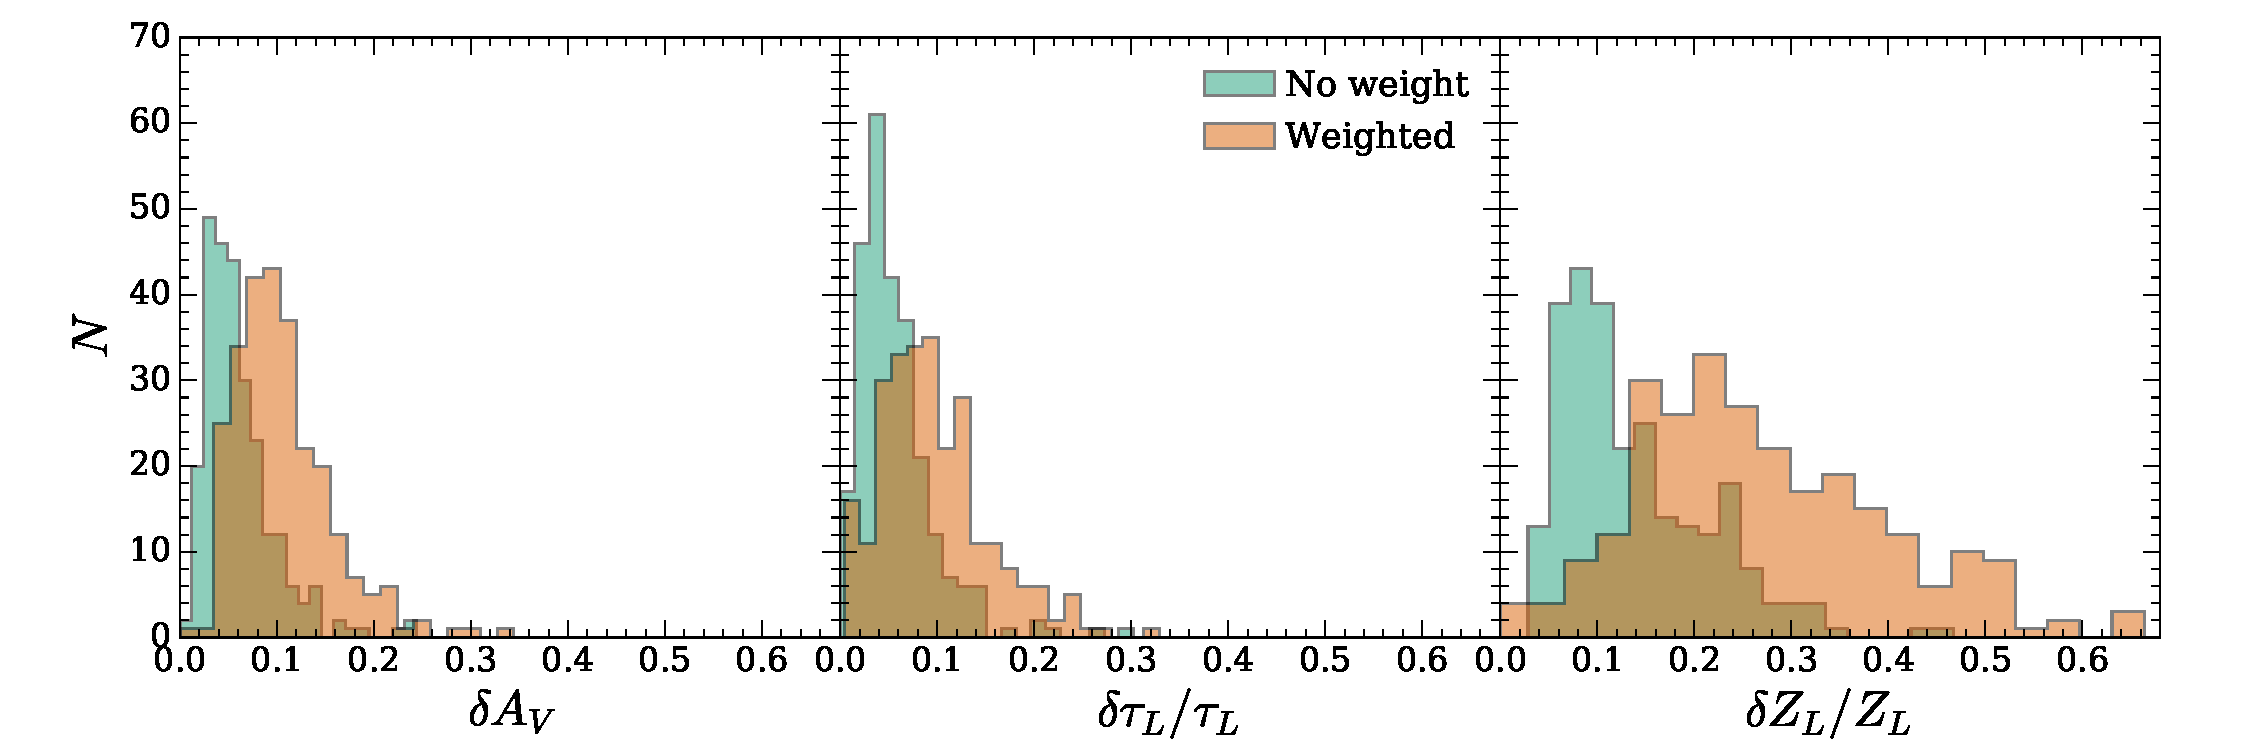
\includegraphics[width=\textwidth]{891_2/figs/weight_comp_hist.pdf}
  \caption[Comparison of uncertainties between weighted and un-weighted
    fits]{\fixspacing\label{891_2:fig:weight_comp}
%% \emph{top:} Derived values of fits
%%     using the weighted $\chi^2$ described in Equation
%%     \ref{891_2:eq:smart_chi} compared to the same values derived using an
%%     un-weighted fit. The dashed lines have a slope of 1. \emph{bottom:}
    Distribution of fitting errors (\S\ref{891_2:sec:fit_err}) for fits
    using un-weighted and weighted $\chi^2$.}
\end{figure*}

%%%%
%ADE: I took out the whole discussion of systematics for now. I think
%it could be interesting, but is not necessary for the argument of why
%we don't use weighted fits.

%% To asses the benefit of using a weighted $\chi^2$ we compare results
%% produced with un-weighted fits to those produced with weighted fits,
%% checking for both systematic differences and the uncertainty distributions
%% of the fits themselves (see \S\ref{891_2:sec:fit_err}). The top
%% panels of Figure \ref{891_2:fig:weight_comp} show the systematic differences
%% between the two schemes. As expected, $A_V$ is highly correlated,
%% indicating that using a weighted $\chi^2$ does not significantly or
%% systematically shift the derived extinction, which speaks to the fact
%% that $A_V$ is mostly driven by the slope of the galaxy SED over a
%% broad wavelength range (although it is also correlated with $\tau_L$,
%% as shown in \S\ref{891_2:sec:fit_err}) and will therefore be relatively
%% insensitive to highly localized changes in $\chi^2$.

%% The middle panel of Figure \ref{891_2:fig:weight_comp} shows that, in many
%% cases, weighted fits find values for $\tau_L$ that are systematically
%% lower than those found via un-weighted fits. This offset is largest
%% for lower values of $\tau_L$, which points to Balmer lines as a likely
%% culprit. In Figure \ref{891_2:fig:RMS_spec} it is clear that the Balmer
%% lines (and in particular \HB, \Hg, and \Hd) are very strong indicators
%% of age and it is likely that the weighted fits increase the fraction
%% of Young SSPs (i.e., lowering the age) to more accurately fit the
%% depth of these lines at the expense of a worse fit in the inter-line
%% continuum where the $\chi^2$ weights are small. 

%% {\bf MAB: This continues to be good discussion. I was wondering if it
%%   is possible to {\it show} your plausible conjecture that the
%%   inter-line regions are not fit a well in the weighted fits, e.g.,
%%   mean spectral residuals. I have a different interpretation of the
%%   middle panel. To my eye the correlation is excellent at the earliest
%%   and youngest ages. At intermediate ages, which just happens to be
%%   where our DFK are probably too coarse, ther is significantly more
%%   scatter.  I don't know what this is telling us but it would be nice
%%   to identify a group of outliers and again compare the mean spectral
%%   residuals between the two classes of fits.}

%% The right panel of Figure \ref{891_2:fig:weight_comp} indicates systematic
%% offsets in $Z_L$ caused by using a weighted $\chi^2$. In particular at
%% low metallicities, as reckoned by the weighted fits, the weighted fits
%% produce systematically lower values while at high metallicities (again
%% weighted by the weighted fit) the weighted fits produce systematically
%% higher values. Many of the strong metallicity indicators shown in
%% Figure \ref{891_2:fig:RMS_spec} have relatively weak amplitudes when
%% compared the uncertainty in the flux values (i.e., they have a low
%% signal to noise) and by increasing the weight in these regions we are
%% possibly pushing $\chi^2$ beyond the limits of our uncertainty. When
%% the signal in one of these metal lines is strong (i.e. high
%% metallicity) the weighted fit will attempt to accurately match the
%% depth of the feature by increasing the fraction of metal-rich SSPs
%% beyond what we be allowed by an un-weighted fit (which is relatively
%% more constrained by the ``featureless'' continuum). When there is very
%% little signal in the metal lines, however, the weighted fits are
%% forced to avoid a small level of absorption on the level of the flux
%% uncertainty that would otherwise be allowed in the un-weighted
%% fits. In other words, in the weighted fits weak metal absorption lines
%% cannot ``hide in the noise'' and therefore a lower total metallicity
%% is needed.

%% {\bf MAB: This needs to be articulated more clearly: ``we are possibly
%%   pushing $\chi^2$ beyond the limits of our uncertainty.'' I didn't
%%   follow your subsequent examples. Even with the weights, there are
%%   many lines. Noise will not make all of them artificially high or
%%   low. So why the systematic difference? And which do you think is
%% right?}

To asses the benefit of using a weighted $\chi^2$ we compare fitting
uncertainties (\S\ref{891_2:sec:fit_err}) produced by un-weighted fits to
those produced with weighted fits and find, somewhat surprisingly,
that a weighted $\chi^2$ produces significantly less precise fits.
Figure \ref{891_2:fig:weight_comp} shows that for all parameters of interest
the distribution of fit uncertainties is larger for weighted fits than
for un-weighted fits, often by a factor of $>$ 2. This level of
uncertainty is unacceptable and it is clear that weighted fits
\emph{do not} improve our ability to understand NGC 891. They are
therefore abandoned for the remainder of this work. We would like to
note, however, that these tests are in no way an exhaustive
exploration of the general concept of weighted $\chi^2$ and we
encourage future research in this topic.

%-------------------
%% {\bf MAB: We are going to need to do a better job here justifying this
%%   section. I want us to keep it in for the final paper; it should
%%   definiely be in the thesis, even as is.  For the paper we need more
%%   work.

%% The key issue that I think we have not fleshed out enough
%% is consideration of accuracy. What we have shown definitively is
%% that weighting reduces precision. This is surprising because we
%% thought we were up-weighting the regions where the astrophysical variance 
%% (which is our ``signal'') was largest. In the above paragraph you 
%% are starting to get at the key issue, namely with statements about
%% systematic differences (could be related to different accuracy) relative
%% to random errors. We need to do two things.

%% (1) Quantify and illustrate the level of systematics vs increased
%% random error (we've only done the latter).

%% How do the projections of $Z_L$, $\tau_L$ and $A_V$ compare for the
%% two fitting methods? Can we say one looks more astrophysically
%% plausible than another? Even if no, this is important to know. Let's
%% make the plots and look at them. Maybe one set w/ two colors for
%% points -- unless we also want to look at height and radius trends.

%% (2) Identify ways to assess if we think one method is more accurate
%% (in the mean) than the other.

%% I would start by looking at the mean residuals for the different fit
%% cases.  As noted above, we may want to do this for subsets of the data
%% where systematics in age and Z are most pronounced. It would be nice
%% to see of the scatter is different in the up-weighted vs down-weighted
%% areas, but I think the key is to identify if one fitting method
%% systematiclly over or under-estimates features or continuum.

%% Where I think we should be going with (1) and (2): While the weighted
%% fits may be noiser, it may be that they are more accurate in the
%% mean. If so this mean provides a possible systematic correction we
%% could apply to the un-weighted fits IF we thought there was some
%% reasonable way to do this. (It will depend on what we find in (1)
%% above.) If we cannot conclude that one fitting method vs the other is
%% plausibly more accurate, then at least we have quantified one
%% assessment of potential systematics in our fitting. That alone
%% justifies the section. In short, you are on the right track; we just
%% need to push it the final step.

%% Wording: ``quantities with larger systematic offsets (i.e., $Z_L$)
%% also have larger fit uncertainty, which dilutes the magnitude of the
%% offset.'' No, it doesn't dilute the magnitude of the offset but its
%% significance.

%% Last two sentences should be revised based on our additional work
%% and/or specific recommendations for future effort (for starters: what
%% we would like to do if we have time.}

%% On the other hand, a full-spectrum fit like that
%% described in \S\ref{891_2:sec:SSP_method} more accurately captures the SED
%% of a galaxy at the expense of strong constraints on the detailed
%% astrophysics. Our RMS-weighted full-spectrum fitting is designed to
%% occupy a middle ground between these two methods. With it we are able
%% to leverage our astrophysical knowledge to focus in on key regions
%% while at the same time fitting all of these regions at once along with
%% the continuum shape. It pretty much rules.
